%    Copyright 2017 Marc Demierre, HES-SO//Master
%
% Licensed under the Apache License, Version 2.0 (the "License");
% you may not use this file except in compliance with the License.
% You may obtain a copy of the License at
%
% http://www.apache.org/licenses/LICENSE-2.0
%
% Unless required by applicable law or agreed to in writing, software
% distributed under the License is distributed on an "AS IS" BASIS,
% WITHOUT WARRANTIES OR CONDITIONS OF ANY KIND, either express or implied.
% See the License for the specific language governing permissions and
% limitations under the License.

% =============================================================================
% | HES-SO//Master - Thesis project report template                           |
% |                                                                           |
% | Originally based on the EPFL template, with many adjustements             |
% =============================================================================

% Document settings
\documentclass[a4paper,11pt,fleqn]{book}
\usepackage[utf8]{inputenc}
\usepackage[T1]{fontenc}
\usepackage[french,english]{babel}

% -----------------------------------------------------------------------------
% Preamble
% -----------------------------------------------------------------------------
% =============================================================================
% | Thesis metadata                                                           |
% =============================================================================

% Thesis info
\newcommand{\ThesisTitle}{GASP: Guide to Assess Security and Privacy levels on web services}
\newcommand{\ThesisSubject}{Master Thesis}
\newcommand{\Orientation}{Information and Communication Technologies (ICT)}
\newcommand{\Keywords}{IT Security, User Privacy, Confidentiality, Web Services, Data Science}

% Author
\newcommand{\AuthorFirstName}{Loïc}
\newcommand{\AuthorLastName}{\textsc{Guibert}}
\newcommand{\AuthorEmail}{loic.guibert@master.hes-so.ch}
\newcommand{\AuthorEmailBackup}{loicguib@ik.me}
\newcommand{\Author}{\AuthorFirstName\ \AuthorLastName}

% First Advisor
\newcommand{\SupervisorOneFirstName}{Pascal}
\newcommand{\SupervisorOneLastName}{\textsc{Bruegger}}
\newcommand{\SupervisorOneSchool}{HES-SO//Master}
\newcommand{\SupervisorOneResearchUnit}{HEIA-FR · iCoSys}
\newcommand{\SupervisorOne}{Dr. \SupervisorOneFirstName\ \SupervisorOneLastName}

% Second Advisor
\newcommand{\SupervisorTwoFirstName}{Adriana}
\newcommand{\SupervisorTwoLastName}{\textsc{Wilde}}
\newcommand{\SupervisorTwoSchool}{University of Winchester · WINTS}
\newcommand{\SupervisorTwoResearchUnit}{University of Southampton · CHT}
\newcommand{\SupervisorTwo}{Dr. \SupervisorTwoFirstName\ \SupervisorTwoLastName}

% Main expert
\newcommand{\ExpertFirstName}{Robert} 
\newcommand{\ExpertLastName}{\textsc{Van Kommer}} 
\newcommand{\Expert}{Dr. \ExpertFirstName\ \ExpertLastName}
\newcommand{\ExpertLab}{EPFL Innovation Park · Alliance}

% Internal expert
\newcommand{\ExpertInternalFirstName}{Jean} 
\newcommand{\ExpertInternalLastName}{\textsc{Hennebert}} 
\newcommand{\ExpertInternal}{Dr. \ExpertInternalFirstName\ \ExpertInternalLastName}

% Advisor
\newcommand{\Advisor}{Philippe \textsc{Joye}}

% Dean
\newcommand{\Dean}{Dr. Bernard \textsc{Masserey}}

% Place (for date and place)
\newcommand{\Date}{\today}
\newcommand{\Place}{Winchester (UK)}

\newcommand{\Researchquestion}{How to help organizations to evaluate their web services that also use \gls{ai} processes, by measuring the risk levels of both \gls{ict} security and user privacy concerns?}         % your project data
% ==================
% Template settings
% ==================

% General tools
% -------------
\usepackage{etoolbox}

% Page style
% ----------
\usepackage[margin=3cm, left=3.5cm, right=3.5cm, twoside=true]{geometry}
\usepackage{fancyhdr}
\setlength{\headheight}{14pt}
\renewcommand{\sectionmark}[1]{\markright{\thesection\ #1}}
\pagestyle{fancy}

% Standard pages (inside chapters)
\fancyhf{}
\renewcommand{\headrulewidth}{0.4pt}
\renewcommand{\footrulewidth}{0pt}
\fancyhead[OR]{\bfseries \nouppercase{\rightmark}}
\fancyhead[EL]{\bfseries \nouppercase{\leftmark}}
\fancyfoot[EL,OR]{\thepage}

% First page of chapters
\fancypagestyle{plain}{
	\fancyhf{}
	\renewcommand{\headrulewidth}{0pt}
	\renewcommand{\footrulewidth}{0pt}
	\fancyfoot[EL,OR]{\thepage}
}

% Imports for external PDFs
\fancypagestyle{addpagenumbersforpdfimports}{
	\fancyhead{}
	\renewcommand{\headrulewidth}{0pt}
	\fancyfoot{}
	\fancyfoot[RO,LE]{\thepage}
}

% Use empty style for page when clearing double pages
\def\cleartoodd{%
	\clearpage%
	\ifodd\value{page}\else\mbox{}\thispagestyle{empty}\newpage\fi%
}

\def\clearchap{%
	\ifodd\value{page}\else\mbox{}\thispagestyle{empty}\fi%
}

% \cleardoublepage replaced by \cleartoodd
\let\origdoublepage\cleardoublepage
\renewcommand{\cleardoublepage}{%
	\cleartoodd%
}

% Fonts
% -----

% Helvetica (Arial used in the MSE Word template)
\usepackage{helvet}

% Math
% ----
\usepackage{amsmath}  % better math

% Floats and figures
% ------------------
\usepackage{newfloat}          % floats
\usepackage[twoside]{caption}  % captions
\usepackage{subcaption}        % subcaptions
\usepackage[section]{placeins} % allows to put float barriers

% Float captions in italics, with label in margin
\DeclareCaptionLabelFormat{title}{#1 #2}
\DeclareCaptionLabelFormat{hangout}{\llap{#1 #2\hspace{5mm}}}
\captionsetup{
	format=hang,
	labelformat=hangout,
	singlelinecheck=false,
	font={it}
}

% Caption with source for figure
% TODO: improve this to use square brackets like the normal "caption"
\newcommand*{\captionsource}[3]{%
\caption[{#1}]{%
	#2%
	
	\textbf{Source:} #3%
}%
}

% Tables
% ------
\usepackage{booktabs} % much better tables
\usepackage{multirow} % allows to fuse rows
\usepackage{array}    % manipulate array
\usepackage{tabularx} % better tables

% Define new tabularx column types:
%  - R: streteched right aligned
%  - C: stretched centered
%  - N: left aligned, specified space
\newcolumntype{R}{>{\raggedleft\arraybackslash}X}%
\newcolumntype{C}{>{\centering\arraybackslash}X}%
\newcolumntype{N}[1]{>{\raggedleft\arraybackslash}p{#1}}

% Set row height multiplicator to provide more breathing space
\renewcommand{\arraystretch}{1.3} 

% Bibliography
% -------------------

% Use biber, with numeric style and no sorting (citation order)
\usepackage[
backend=biber,
style=numeric,
sorting=none,
bibencoding=auto
]{biblatex}
\addbibresource{03-tail/bibliography.bib}


% Tables of contents, figures, tables and listings
% ------------------------------------------------
\usepackage{tocloft}
\newlistof{listing}{lol}{List of Listings}
\setcounter{tocdepth}{1} % Depth to 'section'
\setlength{\cftfigindent}{0pt}  % remove indentation from figures in lof
\setlength{\cftfignumwidth}{1cm}
\setlength{\cfttabindent}{0pt}  % remove indentation from tables in lot
\setlength{\cfttabnumwidth}{1cm}
\setlength{\cftlistingindent}{0pt}
\setlength{\cftlistingnumwidth}{1cm}

% Mini tables of contents
% -----------------------
\usepackage{minitoc}

% no "Contents" title
\mtcsettitle{minitoc}{Contents} 

% Layout
\setlength{\mtcindent}{-0.5em}
\mtcsetoffset{minitoc}{-1em}

% Spacing above and below table
\mtcsetfeature{minitoc}{before}{\vspace{0.5cm}}
\mtcsetfeature{minitoc}{after}{\vspace{-0.25cm}}
\renewcommand{\mtifont}{\sffamily\bfseries\large}
\renewcommand{\mtcSfont}{\sffamily\bfseries\small}
\renewcommand{\mtcSSfont}{\sffamily\small}
\renewcommand{\mtcSSSfont}{\sffamily\small}

% Colors & graphics
% -----------------
\usepackage[table]{xcolor}    % colors
\usepackage[pdftex]{graphicx} % graphics importing
\graphicspath{{02-main/figures/}}
\definecolor{gray80}{gray}{0.80}


% Code and syntax highlighting
% ----------------------------
\usepackage[newfloat]{minted}   % code highlighting

% Typography
% ----------
\usepackage{csquotes}                    % paragraph indentation and spacing
\usepackage[defaultlines=3,all]{nowidow} % avoid widows and orphans
\usepackage{microtype}                   % typographic improvements
\usepackage{parskip}                     % No indent and auto-space between paragraphs
\usepackage[super]{nth}

\usepackage{paralist}
\usepackage{enumitem}
%\setlist{after=\vspace{\baselineskip}} % Modified

% Section and chapters headings
% -----------------------------
\usepackage[explicit]{titlesec} % titles formatting
%\usepackage{titletoc} % titles formatting in ToC etc
%\usepackage{sectsty}  % sectioning commands

% -- Chapters --
% Remove "Chapter N" and use a sans-serif font

% Set layout lengths
\setlength{\headheight}{8mm}
\setlength{\footskip}{1.5cm}
\addtolength{\textheight}{-.5cm}

\titlespacing{\chapter}{-5mm}{-10mm}{3mm}
\titlespacing{\section}{-5mm}{3mm}{-2mm}
\titlespacing{\subsection}{-5mm}{2mm}{-2mm}
\titlespacing{\subsubsection}{-5mm}{2mm}{-1mm}


%\titleformat{\chapter}[block]
%{\Huge}
%{\thechapter\hspace{12pt}\textcolor{gray80}{|}\hspace{12pt}}
%{0pt}
%{\Huge\bfseries}

\titleformat{\chapter}{\Huge\bfseries}{\llap{\thechapter\hspace{12pt}\textcolor{gray80}{|}}}{0mm}{%
	\hfill\begin{minipage}[t]{\dimexpr\textwidth}\raggedright#1\end{minipage}%
}
\titleformat{\section}{\Large\bfseries}{\llap{\thesection}}{0mm}{%
	\hfill\begin{minipage}[t]{\dimexpr\textwidth}\raggedright#1\end{minipage}%
}
\titleformat{\subsection}{\large \bfseries}{\llap{\thesubsection}}{0mm}{%
	\hfill\begin{minipage}[t]{\dimexpr\textwidth}\raggedright#1\end{minipage}%
}
\titleformat{\subsubsection}{\bfseries}{\llap{\thesubsubsection}}{0mm}{%
	\hfill\begin{minipage}[t]{\dimexpr\textwidth}\raggedright#1\end{minipage}%
}

% Misc
% ------
\usepackage{lipsum}    % filler text
\usepackage{blindtext} % random text
\usepackage{lscape}    % easy landscape pages
\usepackage{pdflscape} % landscape pages for PDFs

% Allow email typesetting
\newcommand{\email}[1]{
	\href{mailto:#1}{\textit{#1}}
}

% References
% -----------
\usepackage{url}

 %pdf metadata
\usepackage{hyperref}
\hypersetup{pdftitle={\ThesisTitle},pdfauthor={\Author},pdfsubject={\ThesisSubject},pdfkeywords={\Keywords}}

% % Hyperlinks
% \hypersetup{
% 	colorlinks=true,
% 	linkcolor=black,
% 	citecolor=black,
% 	filecolor=black,
% 	urlcolor=black,
% }

\providecommand*{\listingautorefname}{Listing}


% Glossary
% --------
\usepackage[xindy,toc]{glossaries}
% ==============================================================================
% = Personal glossary of Loïc Guibert, free to use. Used across several projects
% ==============================================================================


% Terms
% -----
% format:  \newglossaryentry{<label>}{<settings>}
% example: \newglossaryentry{computer}
%{
%	name=computer,
%	description={is a programmable machine that receives input,
%		stores and manipulates data, and provides
%		output in a useful format}
%}

\newglossaryentry{backend}{
  name={backend},
  description={The part of a software program that includes its logic layer, which is to generate one or more results from operations. Not visible to users}
}
\newglossaryentry{blockchain}{
	name={blockchain},
	description={A dynamic list of data grouped in \textit{blocks} linked by cryptography mechanisms. Each block brings additional data to the chain and validates the previous block's integrity}
}

\newglossaryentry{cookie}{
  name={cookie},
  description={A cookie is a pair, composed by a key and a value, that is stored on a client's Web browser. It is linked to one or many websites and are used as way to provide stateful information to the website between visits, such as a session identifier}
}
\newglossaryentry{ciphertext}{
  name={ciphertext},
  description={A term used to describe any \gls{plaintext} that has been encryptedby an algorithm. It is not readable without a prior decryption process}
}
\newglossaryentry{cloud}{
  name={cloud},
  description={An architectural model where computing resources are made available to the user without direct active management. Usually describes data centres that are accessible to many users over the Internet}
}
\newglossaryentry{cluster}{
  name={cluster},
  description={A set of computers that work together. Each node have the same task and the whole set can be viewed as a single system}
}

\newglossaryentry{framework}{
	name={framework},
	description={A framework is a set of software components used to bring new possibilities for the development of an IT tool, especially by providing elements related to its infrastructure. Outside of the \gls{it} field, it describes a set of rules, practices or must-haves in order to achieve a goal}
}
\newglossaryentry{frontend}{
  name={frontend},
  description={The part of a software program that includes its graphical presentation layer, which is presented to users}
}

\newglossaryentry{json}{
  name={JSON},
  description={JavaScript Object Notation: a file format widely used for sending information between different information systems. Its structure is very simple and is easily readable by humans}
}

\newglossaryentry{homomorphism}{
  name={homomorphism},
  description={An algebra term which is a mapping between two algebraic structures of the same type}
}

\newglossaryentry{kernel}{
  name={kernel},
  description={One of the fundamental parts of most \glspl{os}. It manages the computer's resources and allows hardware and software components to communicate with each other. One of the most used kernel is \gls{linux}}
}

\newglossaryentry{linux}{
  name={Linux},
  description={Also known as \gls{gnu}/Linux. A family of open source \gls{unix}-like \glspl{os} based on the Linux \gls{kernel}. Numerous Linux distributions have integrated this Linux in their structure and can be used for a wide variety of tasks}
}
\newglossaryentry{lstm}{
  name={Long Short-Term Model},
  description={A \gls{rnn} using units that partially solve the vanishing gradient problem. Allows gradients to flow unchanged if needed}
}

\newglossaryentry{neural network}{
  name={Neural Network},
  description={Network or circuit of artificial neurons that imitates structure of biological brains. It is used for solving artificial intelligence problems}
}
\newglossaryentry{nosql}
{
	name=NoSQL,
	description={Database not using the relational model and the \acrshort{sql} language}
}

\newglossaryentry{opensource}
{
	name={open-source},
	description={The fact to freely share the source code used to build a program to the public, generally associated with a licence. It is also a movement}
}

\newglossaryentry{package_manager}{
  name={package manager},
  description={A package manager is one or several softwares which permit to automate management actions on computer programs. It can install, upgrade, configure and remove them with a understanding of dependencies and compatibility between each others}
}
\newglossaryentry{plaintext}{
  name={plaintext},
  description={A term used to describe any data that is not encrypted and readable by an information system or a human}
}

\newglossaryentry{quic}{
  name={QUIC},
  description={Protocol that aims to replace \gls{tcp} by using some mecanisms from \gls{udp}. Some new features enable better performances, a latency decrease and a non-blocking re-transmission of lost packets}
}

\newglossaryentry{relu}{
  name={ReLU},
  description={An activation function defined as zero for negative inputs and the input value for positive ones. Acts as a ramp function}
}
\newglossaryentry{rest}{
  name={REST},
  description={A set of guidelines for the architecture of an \acrshort{api}, to ensure interoperability between information systems on the Internet}
}
\newglossaryentry{rnn}{
  name={Recurrent Neural Network},
  description={A neural network with connections between nodes that form a directed graph along a temporal sequence}
}

\newglossaryentry{scrum}{
	name={Scrum},
	description={Project management approach that aims to divide the work into sprints, with tasks defined by the team}
}
\newglossaryentry{sgd}{
  name={Stochastic Gradient Descent},
  description={An iterative method for optimizing an objective function with suitable smoothness properties. It can be interpreted as an approximation of the general gradient descent optimization}
}
\newglossaryentry{sigmoid}{
  name={sigmoid},
  description={A function having a S-shaped curve. Often used for probability distribution on a deep-network output layer}
}

\newglossaryentry{tcb}{
    name={TCB},
    description={Includes all hardware, firmware, and software part of a system that are necessary and critical for the system security policy}
}
\newglossaryentry{token}{
    name={token},
    description={A token is a string of characters issued to users by an entity, allowing it to identify the authors of queries within their information system. In general, a token is unique and can be revoked. It is a kind of label, rarely in human-readable form}
}
\newglossaryentry{toolkit}{
    name={toolkit},
    description={Refers to an utility program, several software capabilites or a complete integrated set of software utilities which can be used to develop and maintain applications}
}

\newglossaryentry{unix}{
    name={UNIX},
    description={A family of multi-tasking, multi-user \glspl{os} derived from the original Unix created by \citeproper{AT&T} in the 1970s. It is based on an interpreter or supervisor named the shell and small utilities, each performing a specific action}
}

\newglossaryentry{websocket}{
  name={WebSocket},
  description={A communication protocol that provides full-duplex (bidirectional) communication channels over a single TCP connection. It therefore allows information to be sent to and from servers}
}
\newglossaryentry{white-paper}{
  name={white paper},
  description={A report or guide that present concise information on a complex subject while presenting the author's principles. It is usually intended to facilitate or guide the reader's decision making on the subject, and is used at both institutional and commercial levels}
}



% Acronyms
% --------
% format:  \newacronym{<label>}{<abbrv>}{<full>}
% example: \newacronym{lvm}{LVM}{Logical Volume Manager}
% plural:  \newacronym[longplural={Frames per Second}]{fpsLabel}{FPS}{Frame per Second}

\newacronym{api}{API}{Application Programming Interface}
\newacronym{ai}{AI}{Artificial Intelligence}

\newacronym{ccpa}{CCPA}{California's Consumer Privacy Act}
\newacronym{cep}{CEP}{Complex Event Processing}
\newacronym{ca}{CA}{Certificate Authority}
\newacronym{ci}{CI}{Continuous Integration}
\newacronym{cms}{CMS}{Content Management System}
\newacronym{cqrs}{CQRS}{Command Query Responsibility Segregation}
\newacronym{crud}{CRUD}{Create-Read-Update-Delete}
\newacronym{css}{CSS}{Cascading Style Sheets}

\newacronym{dag}{DAG}{Directed Acyclic Graph}
\newacronym{darpa}{DARPA}{Defense Advanced Research Projects Agency}
\newacronym{dl}{DL}{Deep Learning}
\newacronym{dom}{DOM}{Document Object Model}
\newacronym{dprive}{DPRIVE}{Data Protection in Virtual Environments}
\newacronym{dsl}{DSL}{Domain Specific Language}

\newacronym{eca}{ECA}{Event Condition Action}
\newacronym{elk}{ELK}{Elasticseach Logstash and Kibana}
\newacronym{efk}{EFK}{Elasticseach Fluentd and Kibana}
\newacronym{epa}{EPA}{Event Processing Agent}
\newacronym{epn}{EPN}{Event Processing Network}

\newacronym{fhe}{FHE}{Fully Homomorphic Encryption}
\newacronym{fc}{FC}{Fully Connected}

\newacronym{gdpr}{GDPR}{General Data Protection Regulation }
\newacronym{gelf}{GELF}{Graylog Extended Log Format}
\newacronym{ge}{GE}{Generic Enabler}
\newacronym{gnu}{GNU}{GNU's Not \gls{unix}} %TODO mix glossary and acronym

\newacronym{heia}{HEIA-fr}{School of Engineering and Architecture of Fribourg}
\newacronym{http}{HTTP}{Hypertext Transfer Protocol}
\newacronym{https}{HTTPS}{\glsentryshort{http} Secure}
\newacronym{httpa}{HTTPA}{\glsentryshort{https} Attestable}

\newacronym{ide}{IDE}{Integrated Development Environment}
\newacronym{ietf}{IETF}{Internet Engineering Task Force}
\newacronym{iot}{IoT}{Internet of Things}
\newacronym{ip}{IP}{Internet Protocol}
\newacronym{it}{IT}{Informational Technologies}

\newacronym{jar}{JAR}{Java ARchive}
\newacronym{jmx}{JMX}{Java Management Extensions}
% \newacronym{json}{JSON}{JavaScript Object Notation} TODO: combine with glossary entry
\newacronym{jvm}{JVM}{Java Virtual Machine}

\newacronym{lfhe}{LFHE}{Leveled fully homomorphic encryption}

\newacronym{ml}{ML}{Machine Learning}
\newacronym[longplural={MultiLayer Perceptrons}]
{mlp}{MLP}{MultiLayer Perceptron}
\newacronym{mpc}{MPC}{Multi-Party Computation}
\newacronym{mvc}{MVC}{Model - View - Controller}

\newacronym{npm}{NPM}{Node Package Manager (unofficial name)}
\newacronym[longplural={Neural Networks}]
{nn}{NN}{Neural Network}

\newacronym{os}{OS}{Operating System}
\newacronym{osi}{OSI}{Open Systems Interconnection}

\newacronym{phe}{PHE}{Partially Homomorphic Encryption}
\newacronym{pal}{PAL}{Platform Adaptation Layer}
\newacronym{psp}{PSP}{Platform Security Processor}
\newacronym[longplural={Proofs of Concept}]
{poc}{PoC}{Proof of Concept}

% \newacronym{rest}{REST}{Representational state transfer} TODO: combine with glossary entry
\newacronym{rest_markup}{reST}{reStructuredText}
\newacronym{rfc}{RFC}{Request for Comments}
\newacronym{rpc}{RPC}{Remote Procedure Call}

\newacronym{sdk}{SDK}{Software Development kit}
\newacronym{sgx}{SGX}{Software Guard Extensions}
\newacronym{sql}{SQL}{Structured Query Language}
\newacronym{ssh}{SSH}{Secure Shell}
\newacronym{ssl}{SSL}{Secure Sockets Layer}
\newacronym{swhe}{SWHE}{Somewhat Homomorphic Encryption}

\newacronym{tls}{TLS}{Transport Layer Security}
%\newacronym{tcb}{TCB}{Trusted computing base} TODO: combine with gls
\newacronym{tcp}{TCP}{Transmission Control Protocol}
\newacronym{tdx}{TDX}{Trust Domain Extensions}
\newacronym[
longplural={Trusted Execution Environments}]
{tee}{TEE}{Trusted Execution Environment}
\newacronym{txt-intel}{TXT}{Trusted Execution Technology}
\newacronym{tpm}{TPM}{Trusted Platform Module}

\newacronym{uuid}{UUID}{Universally Unique Identifier}
\newacronym{udp}{UDP}{User Datagram Protocol}
\newacronym{ui}{UI}{User Interface}
\newacronym{uri}{URI}{Universal Resource Identifier}

\newacronym{vm}{VM}{Virtual Machine}

\makeglossaries

    % template settings
% LTeX: enabled=false

% ===========================================
% = Codestyles for minted syntax highlighting
% ===========================================


% How to use (replace 'java' with language name):
% - code blocks:
%     \begin{javacode}
%     CODE
%     \end{javacode}
% - files:
%     full: \javafile{PATH}
%     extract: \javafile[startline=x, endline=y]{PATH}


% Javascript
\newminted{javascript}{frame=single, framesep=6pt, breaklines=true, fontsize=\scriptsize, linenos, autogobble}
\newmintedfile{javascript}{frame=single, framesep=6pt, breaklines=true, 
fontsize=\scriptsize, linenos, autogobble}

% Python
\newminted{python}{frame=single, framesep=6pt, breaklines=true, fontsize=\scriptsize, linenos, autogobble}
\newmintedfile{python}{frame=single, framesep=6pt, breaklines=true, fontsize=\scriptsize, linenos, autogobble}

% Json
\newminted{json}{frame=single, framesep=6pt, breaklines=true, fontsize=\scriptsize, linenos}
\newmintedfile{json}{frame=single, framesep=6pt, breaklines=true, 
	fontsize=\scriptsize, linenos}

% Plain text
\newminted{text}{frame=single, framesep=6pt, breaklines=true, breakanywhere, fontsize=\scriptsize, linenos}
\newmintedfile{text}{frame=single, framesep=6pt, breaklines=true, breakanywhere, fontsize=\scriptsize, linenos}

% LTeX: enabled=true       % code styles for minted
% ========================
% Lighter settings
% ========================

% Marc's font stack
\usepackage{cmbright}       % Sans serif
\usepackage{sourcecodepro}  % Monospace
\renewcommand{\familydefault}{\sfdefault}

\titlespacing{\section}{-5mm}{5mm}{2mm}
\titlespacing{\subsection}{-5mm}{2mm}{1mm}
\titlespacing{\subsubsection}{-5mm}{2mm}{1mm}

% Colors and links - https://en.wikibooks.org/wiki/LaTeX/Hyperlinks
\usepackage{xcolor}% http://ctan.org/pkg/xcolor
\usepackage{hyperref}% http://ctan.org/pkg/hyperref
\hypersetup{
  colorlinks=true,
  linkcolor=blue!50!blue,
  urlcolor=blue!70!blue,
  citecolor=blue!70!blue
%	colorlinks=false,% hyperlinks will be black
%	linkbordercolor=blue,% hyperlink borders will be red
%	pdfborderstyle={/S/U/W 1}% border style will be underline of width 1pt
}

% First acroynm long
\renewcommand*{\CustomAcronymFields}{%
  name={\the\glsshorttok},% name is abbreviated form
  description={\the\glslongtok},% description is long form
  first={\noexpand\emph{\the\glslongtok}\space(\the\glsshorttok)},%
  firstplural={\noexpand\emph{\the\glslongtok\noexpand\acrpluralsuffix}\space(\the\glsshorttok)},%
  text={\the\glsshorttok},%
  plural={\the\glsshorttok\noexpand\acrpluralsuffix}%
}

% To print date in custom command citeproperref
\usepackage[en-GB]{datetime2}

\glsenablehyper

% To continue numbering of footnotes in chapters
% https://tex.stackexchange.com/questions/10448/continuous-footnote-numbering
\counterwithout{footnote}{chapter}

% To suppress errors on custom font sizes
% https://tex.stackexchange.com/questions/58087/how-to-remove-the-warnings-font-shape-ot1-cmss-m-n-in-size-4-not-available
\usepackage{lmodern}

% To import PDF files as content
\usepackage{pdfpages}

% Long tables
\usepackage{ltablex}
\usepackage{booktabs}

% inline citations
\usepackage[
    left = `,%
    right = ',%
    leftsub = ``,%
    rightsub = ''%
]{dirtytalk}

% lighter color
% https://stackoverflow.com/questions/2516976/latex-making-a-lighter-version-of-text-like-anti-bold
\usepackage{color}
\definecolor{light}{rgb}{0.4, 0.4, 0.4}
\def\light#1{{\color{light}#1}}

% change name of the hyperref
% https://tex.stackexchange.com/questions/370991/change-chapter-to-chapter-how-to-do-this-using-autoref/370997#370997
\addto\extrasenglish{%
  \def\chapterautorefname{Chapter}%
  \def\sectionautorefname{Section}%
  \def\subsectionautorefname{Subsection}%
  \def\subsubsectionautorefname{Subsubsection}%
  \def\paragraphautorefname{Paragraph}%
  \def\subparagraphautorefname{Subparagraph}%
}

% Symbols
% https://www.latex4technics.com/?note=22y9
\usepackage{pifont}% http://ctan.org/pkg/pifont
\newcommand{\cmark}{\ding{51}}%
\newcommand{\xmark}{\ding{55}}%

% table spacing 
% https://tex.stackexchange.com/questions/381718/how-to-remove-the-space-after-midrule-in-a-table
\aboverulesep = 0mm \belowrulesep = 0mm  % your custom packages etc
\newcommand{\itembullet}{\begin{itemize}[label={•}]}

\newcommand{\newimage}[4]{
\begin{figure}[!h]
    \begin{center}
        \includegraphics[width=#1\textwidth]{#2}
        \caption{#3}
        \label{fig:#4}
    \end{center}
\end{figure}
}

%TODO Improve with inclusion of the basic form
\newcommand{\newsourcedimage}[8]{
\begin{figure}[!h]
    \begin{center}
        \includegraphics[width=#1\textwidth]{#2}
        %\caption{#3\\\hspace{\textwidth}Source: \url{#4} (accessed \DTMdisplaydate{#5}{#6}{#7}\\)}
        \captionsourcedated{#3}{\url{#4}}{#5}{#6}{#7}
        \label{fig:#8}
    \end{center}
\end{figure}
}

\newcommand{\fullrefname}[1]{\ref{#1} (\nameref*{#1})}
\newcommand{\fullrefnametype}[1]{\autoref{#1} (\nameref*{#1})}
% TODO fix this \newcommand{\Fullrefnametype}[1]{\expandafter\MakeUppercase A}
\newcommand{\Fullrefnametype}[1]{\fullrefnametype{#1}}

\newcommand{\citeproper}[1]{\textit{#1}}
\newcommand{\citeproperref}[5]{\citeproper{#1}\footnote{\textit{#1} source: \url{#2} \accessed{#3}{#4}{#5}}}

% --- Code and minted

% \newenvironment{codeBloc}[3]{
%     \begin{listing}[!ht]
%         \begin{minted}{#1}
%             ...
%         \end{minted}    
%         \caption{#2}
%         \label{listing:#3}
%     \end{listing}
% }

% \newenvironment{codeBloc}[1]
%     {[2]
%     {\end{minted}\caption{#1}\label{listing:#2}\end{listing}}

\newcommand{\codefile}[4]{
    \begin{listing}[!ht]
        \inputminted{#1}{#4}
        \caption{#2}
        \label{listing:#3}
    \end{listing}
}


\newcommand*{\captionsourcedated}[5]{%
\caption[{#1}]{%
	#1%
	
    \textit{Source:} #2%
    \
    \accessed{#3}{#4}{#5}%
	}%
}


\newcommand{\accessed}[3]{%
(accessed \DTMdisplaydate{#1}{#2}{#3}\\)
}         % custom commands

\begin{document}
% -----------------------------------------------------------------------------
% Front matter
% -----------------------------------------------------------------------------
\frontmatter

\dominitoc

% ==========================================================================
% = HES-SO Master thesis title page (modeled after Word template, 2016-2017)
% ==========================================================================

\begin{titlepage}
\newgeometry{margin=2.5cm}
{\fontfamily{phv}\fontseries{mc}\selectfont
	\begin{flushright}
		\begin{minipage}{0.33\textwidth}
			\begin{flushleft}
				
\includegraphics[width=1\textwidth]{img/mse_logo}
			\end{flushleft}
		\end{minipage}%
		\begin{minipage}{0.34\textwidth}
			\begin{center}
				
\includegraphics[width=1\textwidth]{img/hesso_logo.png}
			\end{center}
		\end{minipage}%
		\begin{minipage}{0.33\textwidth}
			\begin{flushright}
				
\includegraphics[width=1\textwidth]{img/winchester_logo}
			\end{flushright}
		\end{minipage}
		\begin{flushleft}
			\footnotesize
			Master of Science HES-SO in Engineering \\
			Av. de Provence 6 \\
			CH-1007 Lausanne
		\end{flushleft}
		~\\[1cm]
		
		{
		\Huge Master of Science HES-SO in Engineering\\[0.5cm]
		}
		
		{
		\LARGE \Orientation\\[1.5cm]
		}
		% Title
		{
			\Huge
			\textbf{\ThesisTitle} \\[0.5cm]
		}
		{
			\LARGE
			Supported by the Department of Digital Technologies \\
			at the University of Winchester, UK \\[1.5cm]
		}
		{
			\large
			\light{Author}\\[-0.3cm]
			\Huge \Author \\[1.5cm]
		}
		{
			\large
			\light{Supervisors} \\
			\SupervisorOne \\
			\textit{\SupervisorOneSchool, \\ \SupervisorOneResearchUnit} \\
			\light{and} \\
			\SupervisorTwo \\
			\textit{\SupervisorTwoSchool, \\ \SupervisorTwoResearchUnit} \\[0.5cm]
		}
		{
			\large
			\light{External expert} \\
			\Expert \\
			\textit{\ExpertLab}
		}
		
		\vfill
		
		% Bottom of the page
		{\large \Place, HES-SO//Master, \Date}
		
	\end{flushright}
}
\restoregeometry
\end{titlepage}

% Table of contents
\cleardoublepage
\phantomsection
\addcontentsline{toc}{chapter}{Contents}
\tableofcontents

% List of figures
\cleardoublepage
\phantomsection
\addcontentsline{toc}{chapter}{List of Figures}
\listoffigures

% Restore paragraphs
\setlength{\parskip}{1em}

% Bold fonts for sections in minitoc
\renewcommand{\cftsecfont}{\sffamily\bfseries}
\renewcommand{\cftsecleader}{\sffamily\bfseries\cftdotfill{\cftdotsep}}
\renewcommand{\cftsecpagefont}{\sffamily\bfseries}


% -----------------------------------------------------------------------------
% Main matter
% -----------------------------------------------------------------------------
\mainmatter

% Chapters
\setcounter{mtc}{6} % Help minitoc skip the front matter chapters
\chapter{Introduction}
\label{chap:introduction}

This specifications document describes all the elements necessary to understand the characteristics of the Master Thesis that takes place in the \citeproper{HES-SO//Master} curriculum.

A Master thesis takes place at the end of all the Master lectures during a whole semester. An amount of nine hundred hours must be dedicated to this end and at least one weekly meeting must be organized through the whole project duration.

This thesis will be realized in collaboration between the \citeproper{HES-SO//Master} and the \citeproper{University of Winchester}. The student will realize his thesis abroad, at the city of Winchester.

In this document will be explained the context, objectives, activities and planning of the thesis.

All the documents produced during this project will be stored on the \gls{heia} software forge\cite{website:gitlab}.
\newpage
\chapter{Context}
\label{chap:context}

This chapter will describe the context around the subject of the thesis. We will explain the actual state that contains a problem to be solved, and the author's contribution that will contribute to fix the previously described problem. We will also introduce the different actors that will intervene during the thesis.

% -----------------------------------------------------------------------------
\section{Actual State}
\label{sec:context_actual}

In a world where \gls{it} security is increasingly valuable and necessary, the need for new ways to secure and trust information systems is growing. This need is particularly expressed in the \gls{ai} field, where big amounts of data are periodically collected in order to improve services performances or to monetize them. Furthermore, such data is often personal and highly related to their user, which raise ethical and privacy-related questions.

Nowadays, end users of public or private online services are more and more aware of personal data related risks and a change in consumption patterns is being noticed. Therefore, new approaches for the whole \gls{it} field must be developed in order to provide secured and privacy-first online services that can nevertheless enable a personalized experience.

% -----------------------------------------------------------------------------
\section{Contribution}
\label{sec:context_contribution}

By enabling secured and privacy-oriented personalized experience on online services, companies would be able to provide ethical, modern and respectful offers to their customers. All stakeholders would benefit from such implementations, as long as the performance, time or processing capabilities do not restraint them in their activities.

This thesis aims to provide which technologies, best practices or safeguards can be integrated to information systems in order to ensure secured environments to the end users, particularly regarding AI projects. These components must then be implemented in a functional information system, which includes \gls{ai} processes, while providing a conclusion on the changes of such integration compared to the initial information system.

We want to offer a suitable solution to those wishing to increase the security and confidentiality of their online services. A focus will also be made on the \gls{ai} field.

% -----------------------------------------------------------------------------
\section{Actors}
\label{sec:context_actors}

The thesis will be conducted by \Author.

There are two advisors for this thesis: \AdvisorOne \ and \AdvisorTwo. 

The thesis subject has been proposed by \Author \ as a personal project and is related to the field of research of the two advisors. A secured online service is being developed by \AdvisorOne \ and includes aspects similar to this thesis subject.

An expert will be assigned to the thesis in order to evaluate it when completed and returned. This assignment will be made later during the semester.
\newpage
\chapter{Objectives}
\label{chap:objectives}

Following the enumeration made in \fullrefname{sec:context_contribution}, questions need to be asked in order to complete this project.
\begin{itemize}
    \item Which rules, best practices, technologies and aspects should be used in order to improve the security and confidentiality of online services?
    \item Which specific rules, best practices, technologies and aspects should be used in order to improve the security and confidentiality of the \gls{ai} field, particularly for \gls{ml} and \gls{dl} models?
    \item How can we provide an understandable and complete model of our findings?
\end{itemize}

The objectives below intent to provide answers to the questions asked.

% -----------------------------------------------------------------------------
\section{Primary Objectives}
\label{sec:objectives_primary}

All those objectives must be fulfilled in order to successfully complete the thesis.

\subsection{Establish an Up-To-Date Knowledge Collection}
\label{sec:objectives_primary_knowledge}

We need to collect an up-to-date and complete knowledge of the rules, best practices, technologies and aspects that contribute to enforce the security and privacy of online services. To this end, a proper literature review must be conducted. Its results will then be used as a foundation for the next phase of the thesis.

The content related to this objective must be included into the thesis report. It will list, explain and analyse the concepts found during the collection.

This objective must be completed before the end of the thesis, which is the \DTMdisplaydate{2023}{2}{10}{}.

\subsection{Provide an Understandable Guide or \Gls{framework}}
\label{sec:objectives_primary_guide}

Using the previously collected knowledge about security and privacy, a guide or \gls{framework} must be built. It must provide an understandable and appliable methodology in order to evaluate online services.

The content related to this objective must be included into the thesis report. It will list, explain and analyse the methodology used to build the guide or \gls{framework} and its content. The result of this objective will be an independent document, which must be attached to the thesis report as an appendix.

This objective must be completed before the end of the thesis, which is the \DTMdisplaydate{2023}{2}{10}{}.

\subsection{Apply and Test the Guide or \Gls{framework} on an Online Service}
\label{sec:objectives_primary_test}

Proper metrics must be used in order to conduct a proper evaluation of the guide or \gls{framework}. Once defined and explained, an evaluation of an online service including one or more \gls{ai} processes will be made, and the results will then be analysed and discussed.

The online service should be accessible and open, which means that we should have access to the source code. To this end, we could use the \citeproperref{Hestia}{https://bit.ly/3BzeDSN}{2022}{09}{22} ecosystem, which is an ongoing project leaded by \AdvisorOne.

The content related to this objective must be included into the thesis report. It will explain and analyse the results obtained during the evaluation.

This objective must be completed before the end of the thesis, which is the \DTMdisplaydate{2023}{2}{10}{}.

% -----------------------------------------------------------------------------
\section{Secondary Objectives}
\label{sec:objectives_secondary}

The secondary objective will only be completed if all primary objectives have been fulfilled and if there is still time left before the end of the project's timeframe.

\subsection{Submit the Guide as an Online Resource}
\label{sec:objectives_secondary_online}

Because of the nature of this thesis being an academical work and the ethics of such approaches, we believe that publishing the guide or \gls{framework} on the Internet would be useful to the public. It should therefore be published on some online platforms, such as a custom website, a forum or something equivalent.

The content related to this objective must be included into the thesis report. It will explain and analyse the approaches made in order to publish the guide or \gls{framework} online.

If this objective is considered, it must be completed before the end of the thesis, which is the \DTMdisplaydate{2023}{2}{10}{}.

% -----------------------------------------------------------------------------
\section{Constraints}
\label{sec:objectives_constraints}

Apart from the ones described in the respective objectives, an additional constraint must be respected regarding the whole thesis scope.

If any data collected under real-life conditions is used, analysed or processed during this thesis, ethical considerations and obligations must be applied.
\newpage
\chapter{Activities}
\label{chap:activities}

The previously defined objectives imply several work activities in order to fulfil them. These activities are separated into more specific tasks. Please note that those tasks will not necessarily be done in a chronological order.

% -----------------------------------------------------------------------------
\section{Specifications}
\label{sec:activities_specifications}

This activity defines the scope and objectives of the thesis.

\begin{enumerate}
	\item Define the project specification
	\item Define the project planning
\end{enumerate}


% -----------------------------------------------------------------------------
\section{State of the Art}
\label{sec:activities_sota}

This activity covers the \fullrefname{sec:objectives_primary_knowledge} objective.

\begin{enumerate}
	\item Gather scientific articles and papers
	\item Gather online resources
	\item Gather standards
	\item Gather technologies
	\item Assess, analyse and explain the relevant resources
\end{enumerate}


% -----------------------------------------------------------------------------
\section{Methodology}
\label{sec:activities_methodology}

This activity partially covers the \fullrefname{sec:objectives_primary_guide} objective.

\begin{enumerate}
	\item Define and explain the guide or \gls{framework} chosen format
	\item Gather resources for the chosen format
	\item Prepare the document
\end{enumerate}

\newpage

% -----------------------------------------------------------------------------
\section{Build the Guide or \Gls{framework}}
\label{sec:activities_build}

This activity partially covers the \fullrefname{sec:objectives_primary_guide} objective.

\begin{enumerate}
	\item Define the categories
	\item Define the items to evaluate
	\item Define the evaluation process
\end{enumerate}


% -----------------------------------------------------------------------------
\section{Test and Evaluation}
\label{sec:activities_evaluation}

This activity covers the \fullrefname{sec:objectives_primary_test} objective.

\begin{enumerate}
	\item Define the proper metrics to evaluate the guide of \gls{framework}
	\item Get access to an online service
	\item Apply the methodology previously defined
	\item Evaluate and explain the results
\end{enumerate}

% -----------------------------------------------------------------------------
\section{Publish the Guide or \Gls{framework}}
\label{sec:activities_publish}

This activity covers the \fullrefname{sec:objectives_secondary_online} secondary objective.

\begin{enumerate}
	\item Assess the suitable online platforms
	\item Publish the document on selected platform(s).
\end{enumerate}


% -----------------------------------------------------------------------------
\section{Documentation}
\label{sec:activities_documentation}

The thesis report will be realized throughout the duration of the whole project, but this activity will be conducted at its end in order to change last details in said report. A poster must also be produced.

\begin{enumerate}
    \item Produce the thesis poster
    \item Finalize the thesis report
\end{enumerate}
\newpage
\chapter{Planning}
\label{chap:planning}

Around nine hundred hours of work are required for this thesis: this amount depends on the number of indicated credits.

The public holidays are taken into account: one week of break has been planned during winter holidays. Weekends are not included into the planning but can be used to catch up possible delays.

We will work with the \gls{scrum} method, which is an iterative agile method. The duration of the sprints is of one week excepted for exceptions due to special occasions (sprints number 1, 13, 14 and 18), with a backlog definition made at each weekly meeting. The tasks defined in \fullrefname{chap:activities} can be directly included into the backlog or can be divided into smaller tasks.

The major observed differences will be notified into meeting minutes.

\fullrefnametype{fig:ch5_gantt} shows a graphical view of the corresponding planning.

% -----------------------------------------------------------------------------
\section{First Sprint (1st)}
\label{sec:planning_first}

\textbf{Timeline}:
\begin{itemize}
    \item Start - 19.09.2022
	\item End - 28.09.2022
\end{itemize}

\textbf{Activity to complete}:
\begin{itemize}
    \item \fullrefname{sec:activities_specifications}
\end{itemize}

\textbf{Deliverable}:
\begin{itemize}
    \item Specifications document
\end{itemize}

% -----------------------------------------------------------------------------
\section{Second Sprint (2nd)}
\label{sec:planning_second}

\textbf{Timeline}:
\begin{itemize}
    \item Start - 29.09.2022
	\item End - 05.10.2022
\end{itemize}

\newpage

\textbf{Activity to complete}:
\begin{itemize}
    \item \fullrefname{sec:activities_sota}
\end{itemize}

\textbf{Deliverable}: none

% -----------------------------------------------------------------------------
\section{Third Sprint (3rd)}
\label{sec:planning_third}

\textbf{Timeline}:
\begin{itemize}
    \item Start - 06.10.2022
	\item End - 12.10.2022
\end{itemize}

\textbf{Activity to complete}:
\begin{itemize}
    \item \fullrefname{sec:activities_sota}
\end{itemize}

\textbf{Deliverable}: none

% -----------------------------------------------------------------------------
\section{Fourth Sprint (4th)}
\label{sec:planning_fourth}

\textbf{Timeline}:
\begin{itemize}
    \item Start - 13.10.2022
	\item End - 19.10.2022
\end{itemize}

\textbf{Activity to complete}:
\begin{itemize}
    \item \fullrefname{sec:activities_sota}
\end{itemize}

\textbf{Deliverable}: none

% -----------------------------------------------------------------------------
\section{Fifth Sprint (5th)}
\label{sec:planning_fifth}

\textbf{Timeline}:
\begin{itemize}
    \item Start - 20.10.2022
	\item End - 26.10.2022
\end{itemize}

\textbf{Activity to complete}:
\begin{itemize}
    \item \fullrefname{sec:activities_sota}
\end{itemize}

\textbf{Deliverable}: none

% -----------------------------------------------------------------------------
\section{Sixth Sprint (6th)}
\label{sec:planning_sixth}

\textbf{Timeline}:
\begin{itemize}
    \item Start - 27.10.2022
	\item End - 02.11.2022
\end{itemize}

\textbf{Activity to complete}:
\begin{itemize}
    \item \fullrefname{sec:activities_sota}
\end{itemize}

\textbf{Deliverable}: none

% -----------------------------------------------------------------------------
\section{Seventh Sprint (7th)}
\label{sec:planning_seventh}

\textbf{Timeline}:
\begin{itemize}
    \item Start - 03.11.2022
	\item End - 09.11.2022
\end{itemize}

\textbf{Activity to complete}:
\begin{itemize}
    \item \fullrefname{sec:activities_sota}
\end{itemize}

\textbf{Deliverables}: 
\begin{itemize}
    \item An up-to-date state of the art
    \item Report content
\end{itemize}

% -----------------------------------------------------------------------------
\section{Eighth Sprint (8th)}
\label{sec:planning_eigth}

\textbf{Timeline}:
\begin{itemize}
    \item Start - 10.11.2022
	\item End - 16.11.2022
\end{itemize}

\textbf{Activity to complete}:
\begin{itemize}
    \item \fullrefname{sec:activities_methodology}
\end{itemize}

\textbf{Deliverable}: none

% -----------------------------------------------------------------------------
\section{Ninth Sprint (9th)}
\label{sec:planning_ninth}

\textbf{Timeline}:
\begin{itemize}
    \item Start - 17.11.2022
	\item End - 23.11.2022
\end{itemize}

\textbf{Activity to complete}:
\begin{itemize}
    \item \fullrefname{sec:activities_methodology}
\end{itemize}

\textbf{Deliverables}: 
\begin{itemize}
    \item Defined methodology for the guide or \gls{framework}
    \item Report content
\end{itemize}

% -----------------------------------------------------------------------------
\section{Tenth Sprint (10th)}
\label{sec:planning_tenth}

\textbf{Timeline}:
\begin{itemize}
    \item Start - 24.11.2022
	\item End - 30.11.2022
\end{itemize}

\textbf{Activity to complete}:
\begin{itemize}
    \item \fullrefname{sec:activities_build}
\end{itemize}

\textbf{Deliverable}: none

% -----------------------------------------------------------------------------
\section{Eleventh Sprint (11th)}
\label{sec:planning_eleventh}

\textbf{Timeline}:
\begin{itemize}
    \item Start - 01.12.2022
	\item End - 07.12.2022
\end{itemize}

\textbf{Activity to complete}:
\begin{itemize}
    \item \fullrefname{sec:activities_build}
\end{itemize}

\textbf{Deliverable}: none

% -----------------------------------------------------------------------------
\section{Twelfth Sprint (12th)}
\label{sec:planning_twelfth}

\textbf{Timeline}:
\begin{itemize}
    \item Start - 08.12.2022
	\item End - 14.12.2022
\end{itemize}

\textbf{Activity to complete}:
\begin{itemize}
    \item \fullrefname{sec:activities_build}
\end{itemize}

\textbf{Deliverable}: none

% -----------------------------------------------------------------------------
\section{Thirteenth Sprint (13th)}
\label{sec:planning_thirteenth}

\textbf{Timeline}:
\begin{itemize}
    \item Start - 15.12.2022
	\item End - 23.12.2022
\end{itemize}

\textbf{Activity to complete}:
\begin{itemize}
    \item \fullrefname{sec:activities_build}
\end{itemize}

\textbf{Deliverable}: none

\textit{Winter vacations}

% -----------------------------------------------------------------------------
\section{Fourteenth Sprint (14th)}
\label{sec:planning_fourteenth}

\textbf{Timeline}:
\begin{itemize}
    \item Start - 02.01.2023
	\item End - 11.01.2023
\end{itemize}

\textbf{Activities to complete}:
\begin{itemize}
    \item \fullrefname{sec:activities_build}
    \item \fullrefname{sec:activities_evaluation}
\end{itemize}

\textbf{Deliverables}: 
\begin{itemize}
    \item Guide or \gls{framework}
    \item Report content
\end{itemize}

% -----------------------------------------------------------------------------
\section{Fifteenth Sprint (15th)}
\label{sec:planning_fifteenth}

\textbf{Timeline}:
\begin{itemize}
    \item Start - 12.01.2023
	\item End - 18.01.2023
\end{itemize}

\textbf{Activity to complete}:
\begin{itemize}
    \item \fullrefname{sec:activities_evaluation}
\end{itemize}

\textbf{Deliverable}: none

% -----------------------------------------------------------------------------
\section{Sixteenth Sprint (16th)}
\label{sec:planning_sixteenth}

\textbf{Timeline}:
\begin{itemize}
    \item Start - 19.01.2023
	\item End - 25.01.2023
\end{itemize}

\textbf{Activity to complete}:
\begin{itemize}
    \item \fullrefname{sec:activities_evaluation}
\end{itemize}

\textbf{Deliverable}: none

% -----------------------------------------------------------------------------
\section{Seventeenth Sprint (17th)}
\label{sec:planning_seventeenth}

\textbf{Timeline}:
\begin{itemize}
    \item Start - 26.01.2023
	\item End - 01.02.2023
\end{itemize}

\textbf{Activity to complete}:
\begin{itemize}
    \item \fullrefname{sec:activities_evaluation}
\end{itemize}

\textbf{Deliverable}: none

% -----------------------------------------------------------------------------
\section{Eighteenth Sprint (18th)}
\label{sec:planning_eighteenth}

\textbf{Timeline}:
\begin{itemize}
    \item Start - 02.02.2023
	\item End - 08.02.2023
\end{itemize}

\textbf{Activity to complete}:
\begin{itemize}
    \item \fullrefname{sec:activities_evaluation}
\end{itemize}

\textbf{Deliverables}: 
\begin{itemize}
    \item Evaluation of an online service
    \item Report content
\end{itemize}

% -----------------------------------------------------------------------------
\section{Nineteenth Sprint (19th)}
\label{sec:planning_nineteenth}

\textbf{Timeline}:
\begin{itemize}
    \item Start - 09.02.2023
	\item End - 10.02.2023
\end{itemize}

\textbf{Activity to complete}:
\begin{itemize}
    \item \fullrefname{sec:activities_documentation}
\end{itemize}

\textbf{Deliverables}: 
\begin{itemize}
    \item Master poster
    \item Completed master thesis
\end{itemize}

\newpage

\newimage{0.85}{ch5_gantt.png}{Gantt planning of the thesis}{ch5_gantt}
\newpage

% Appendices
\appendix
\chapter{Appendices}

This Chapter provides all the appendixes we mentioned during our thesis. Their original files can be accessed on the thesis repository~\cite{mt-forge} as well.

% -----------------------------------------------------------------------------
\newappendix{Specifications Document}
\label{appendix:specifications}

The next twenty-nine pages present the specifications document that has been defined for this thesis.

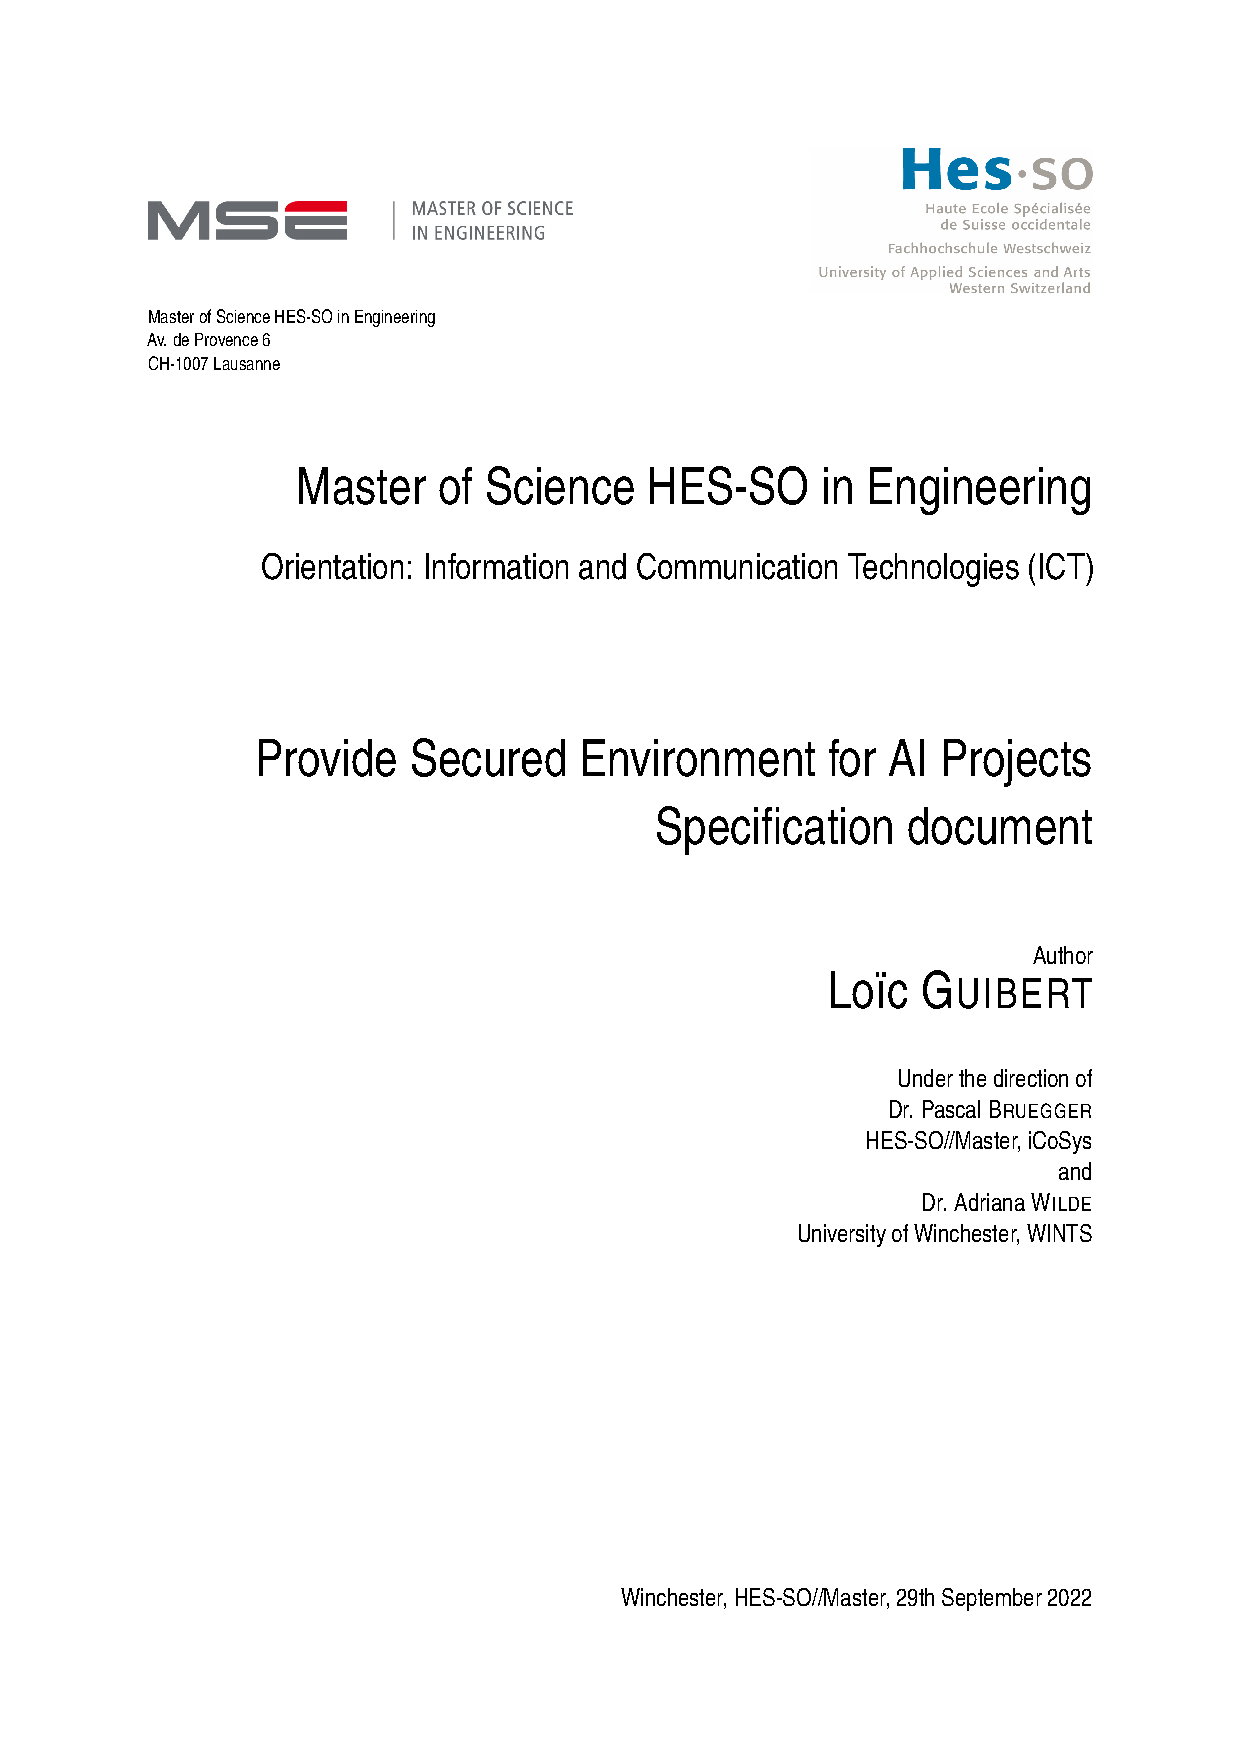
\includepdf[pages=-]{03-tail/appendices/specifications.pdf}

% -----------------------------------------------------------------------------
\newappendix{Guide Content}
\label{appendix:guide}

%TODO
The next fifty pages present the spreadsheet file acting as the dataset that has been defined during this thesis.

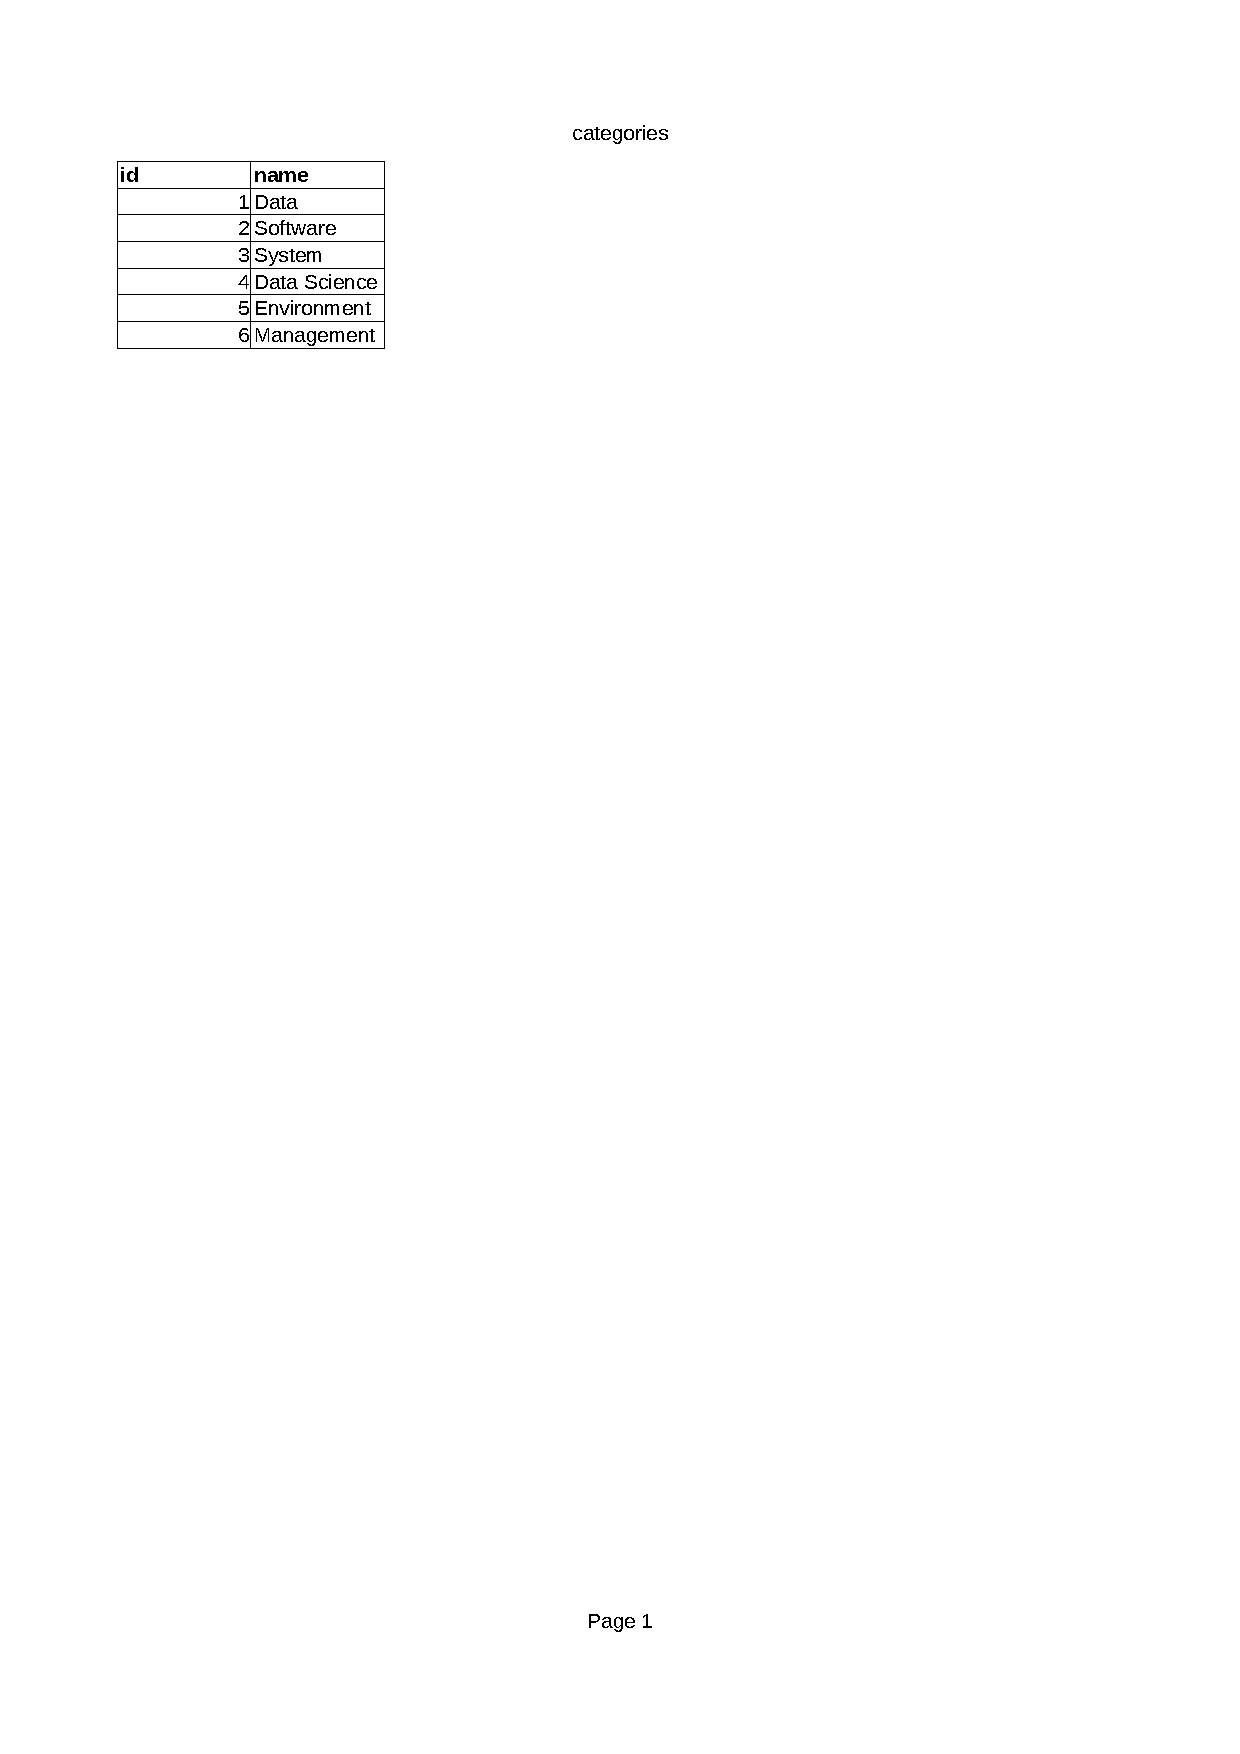
\includepdf[pages={-},fitpaper,rotateoversize]{03-tail/appendices/dataset.pdf}

% -----------------------------------------------------------------------------
\newappendix{Software Tests}
\label{appendix:tests}

\captionsetup[table]{list=no}

% Counters 
\newcounter{testsdatacounter}
\newcounter{testsappcounter}

The results of the conducted software tests are summarized in this appendix.

\begin{hyphenrules}{nohyphenation}
	\begin{table}[ht]
		\begin{center}
			\begin{tabularx}{\textwidth}{l|p{4cm}Xc}
				\toprule[0.8mm]
				\textbf{ID} & \textbf{Action} & \textbf{Expected result} & \textbf{Result} \\
				\midrule[0.8mm] 
				\stepcounter{testsdatacounter}
				1.\thetestsdatacounter & Run script with valid arguments & The arguments are passed to the script and used by it & \cellcolor{green!25}OK \\
				\midrule 
				\stepcounter{testsdatacounter}
				1.\thetestsdatacounter & Run script with invalid arguments & The script exits after showing the arguments & \cellcolor{green!25}OK \\
				\midrule 
				\stepcounter{testsdatacounter}
				1.\thetestsdatacounter & Run script without arguments & The script exits after showing the arguments & \cellcolor{green!25}OK \\
				\midrule 
				\stepcounter{testsdatacounter}
				1.\thetestsdatacounter & Run script with the \texttt{help} argument & The script exits after showing the arguments & \cellcolor{green!25}OK \\
				\midrule 
				\stepcounter{testsdatacounter}
				1.\thetestsdatacounter & Run script with as invalid \citeproper{ODS} file & The script exits after showing the reason & \cellcolor{green!25}OK \\
				\midrule 
				\stepcounter{testsdatacounter}
				1.\thetestsdatacounter & The \citeproper{ODS} file has an invalid attribute & The attribute is not processed & \cellcolor{green!25}OK \\
				\midrule 
				\stepcounter{testsdatacounter}
				1.\thetestsdatacounter & The \citeproper{ODS} file has an invalid value & The script shows the error & \cellcolor{green!25}OK \\
				\midrule 
				\stepcounter{testsdatacounter}
				1.\thetestsdatacounter & The hash is calculated based on the guide content & The hash is valid & \cellcolor{green!25}OK \\
				\bottomrule[0.8mm]
			\end{tabularx}
		\end{center}
		\caption*{Data conversion tests}
	\end{table}
\end{hyphenrules}

\begin{table}[ht]
    \begin{center}
        \begin{tabularx}{\textwidth}{l|XXc}
            \toprule[0.8mm]
            \textbf{ID} & \textbf{Action} & \textbf{Expected result} & \textbf{Result} \\
            \midrule[0.8mm] 
			\stepcounter{testsappcounter}
            2.\thetestsappcounter & Click on the evaluation button. & The \texttt{ExplanationView} page opens. & \cellcolor{green!25}OK \\
            \midrule 
			\stepcounter{testsappcounter}
            2.\thetestsappcounter & Click on the restoration button. & The \texttt{ResorationView} page opens. & \cellcolor{green!25}OK \\
            \midrule 
			\stepcounter{testsappcounter}
            2.\thetestsappcounter & Click on the report button. & The report \gls{pdf} file opens in another tab. & \cellcolor{green!25}OK \\
            \midrule 
			\stepcounter{testsappcounter}
            2.\thetestsappcounter & Click on the \gls{pwa} browser titles. & Additional installation information is shown. & \cellcolor{green!25}OK \\
            \midrule 
			\stepcounter{testsappcounter}
            2.\thetestsappcounter & Click on the \gls{pwa} links. & Links are opened in another browser tab. & \cellcolor{green!25}OK \\
            \bottomrule[0.8mm]
        \end{tabularx}
    \end{center}
    \caption*{Application tests on the \texttt{HomeView} user interface}
    \label{table:app_tests_ui_homeview}
\end{table}

\begin{hyphenrules}{nohyphenation}
\begin{table}[ht]
    \begin{center}
        \begin{tabularx}{\textwidth}{l|p{3.2cm}Xc}
            \toprule[0.8mm]
				\textbf{ID} & \textbf{Action} & \textbf{Expected result} & \textbf{Result} \\
				\midrule[0.8mm] 
				\stepcounter{testsappcounter}
				2.\thetestsappcounter & Click on the upload form. & A system modal window opens to select a \gls{json} file. & \cellcolor{green!25}OK \\
				\midrule 
				\stepcounter{testsappcounter}
				2.\thetestsappcounter & Click on the upload submit button. & The integrity of the \gls{json} file is verified, the progress or results are saved into the store and the assessor is redirected to either the \texttt{EvaluationView} page or the \texttt{ResultsView} page. & \cellcolor{green!25}OK \\
				\bottomrule[0.8mm]
        \end{tabularx}
    \end{center}
    \caption*{Application tests on the \texttt{RestoreView} user interface}
    \label{table:app_tests_ui_restoreview}
\end{table}
\end{hyphenrules}

\begin{hyphenrules}{nohyphenation}
	\begin{table}[ht]
		\begin{center}
			\begin{tabularx}{\textwidth}{l|p{4cm}Xc}
				\toprule[0.8mm]
				\textbf{ID} & \textbf{Action} & \textbf{Expected result} & \textbf{Result} \\
				\midrule[0.8mm] 
				\stepcounter{testsappcounter}
				2.\thetestsappcounter & Click on the text to change guide content. & Additional information and an upload form are shown. & \cellcolor{green!25}OK \\
				\midrule 
				\stepcounter{testsappcounter}
				2.\thetestsappcounter & Click on the upload form. & A system modal window opens to select a \gls{json} file. & \cellcolor{green!25}OK \\
				\midrule 
				\stepcounter{testsappcounter}
				2.\thetestsappcounter & Click on the upload submit button. & The integrity of the \gls{json} file is verified, the guide content is saved into the store, and the assessor is redirected to the \texttt{EvaluationView} page. & \cellcolor{green!25}OK \\
				\midrule 
				\stepcounter{testsappcounter}
				2.\thetestsappcounter & Click on an item of the guide example. & If at least one description exists for the item, the item expends to give additional information, and collapses back on second click. & \cellcolor{green!25}OK \\
				\midrule 
				\stepcounter{testsappcounter}
				2.\thetestsappcounter & Click on an item checkbox of the guide example. & The store state is not updated. & \cellcolor{green!25}OK \\
				\midrule 
				\stepcounter{testsappcounter}
				2.\thetestsappcounter & Click on the evaluation button. & The \texttt{EvaluationView} page opens. & \cellcolor{green!25}OK \\
				\bottomrule[0.8mm]
			\end{tabularx}
		\end{center}
		\caption*{Application tests on the \texttt{ExplanationView} user interface}
		\label{table:app_tests_ui_explanationview}
	\end{table}
\end{hyphenrules}

\begin{hyphenrules}{nohyphenation}
	\begin{table}[ht]
		\begin{center}
			\begin{tabularx}{\textwidth}{l|p{4cm}Xc}
				\toprule[0.8mm]
				\textbf{ID} & \textbf{Action} & \textbf{Expected result} & \textbf{Result} \\
				\midrule[0.8mm] 
				\stepcounter{testsappcounter}
				2.\thetestsappcounter & Click on a subcategory name in the \texttt{Sidebar}. & Objectives, items and descriptions of the subcategory are displayed. & \cellcolor{green!25}OK \\
				\midrule 
				\stepcounter{testsappcounter}
				2.\thetestsappcounter & Click on the close option in the expended \texttt{Sidebar}. & The \texttt{Sidebar} is hidden. & \cellcolor{green!25}OK \\
				\midrule 
				\stepcounter{testsappcounter}
				2.\thetestsappcounter & Click on the expend icon to collapse the \texttt{Sidebar}. & The \texttt{Sidebar} is expended. & \cellcolor{green!25}OK \\
				\midrule 
				\stepcounter{testsappcounter}
				2.\thetestsappcounter & Click on a collapsed category in the \texttt{Sidebar}. & The group containing children of the category is expended. & \cellcolor{green!25}OK \\
				\midrule 
				\stepcounter{testsappcounter}
				2.\thetestsappcounter & Click on an expended category in the \texttt{Sidebar}. & The group containing children of the category is collapsed. & \cellcolor{green!25}OK \\
				\midrule 
				\stepcounter{testsappcounter}
				2.\thetestsappcounter & Click on the results button in the \texttt{Sidebar}. & If the evaluation is complete, the \texttt{ResultsView} page opens. & \cellcolor{green!25}OK \\
				\midrule 
				\stepcounter{testsappcounter}
				2.\thetestsappcounter & Click on the saving button in the \texttt{Sidebar}. & A \gls{json} file is downloaded containing the evaluation progress and the guide content. & \cellcolor{green!25}OK \\
				\midrule 
				\stepcounter{testsappcounter}
				2.\thetestsappcounter & Click on an item. & If at least one description exists for the item, the item expends to give additional information, and collapses back on second click. & \cellcolor{green!25}OK \\
				\midrule 
				\stepcounter{testsappcounter}
				2.\thetestsappcounter & Click on an item checkbox. & The store state is updated, and the checkbox is updated with the corresponding state value. & \cellcolor{green!25}OK \\
				\midrule 
				\stepcounter{testsappcounter}
				2.\thetestsappcounter & Click on an item checkbox. & The evaluation values change accordingly (unchecked to compliant, compliant to non-compliant, non-compliant to not concerned, not concerned to compliant). & \cellcolor{green!25}OK \\
				\midrule 
				\stepcounter{testsappcounter}
				2.\thetestsappcounter & Click on a description link. & Links are opened in another browser tab. & \cellcolor{green!25}OK \\
				\midrule 
				\stepcounter{testsappcounter}
				2.\thetestsappcounter & The last item of a subcategory is evaluated. & The corresponding subcategory is shown as completed in the \texttt{Sidebar}. & \cellcolor{green!25}OK \\
				\midrule 
				\stepcounter{testsappcounter}
				2.\thetestsappcounter & The last item of a category is evaluated. & The corresponding category is shown as completed in the \texttt{Sidebar}. & \cellcolor{green!25}OK \\
				\midrule 
				\stepcounter{testsappcounter}
				2.\thetestsappcounter & The last item of the guide is evaluated. & The result button is activated. & \cellcolor{green!25}OK \\
				\bottomrule[0.8mm]
			\end{tabularx}
		\end{center}
		\caption*{Application tests on the \texttt{EvaluationView} user interface}
		\label{table:app_tests_ui_evaluationview}
	\end{table}
\end{hyphenrules}

\begin{table}[ht]
    \begin{center}
        \begin{tabularx}{\textwidth}{l|XXc}
            \toprule[0.8mm]
            \textbf{ID} & \textbf{Action} & \textbf{Expected result} & \textbf{Result} \\
            \midrule[0.8mm] 
			\stepcounter{testsappcounter}
            2.\thetestsappcounter & If displayed, click on the non-compliant button. & The page scrolls to the non-compliant items. & \cellcolor{green!25}OK \\
			\midrule 
			\stepcounter{testsappcounter}
            2.\thetestsappcounter & Click on the download button. & A \gls{json} file is downloaded containing the evaluation progress and the guide content. & \cellcolor{green!25}OK \\
			\midrule 
			\stepcounter{testsappcounter}
			2.\thetestsappcounter & Click on the evaluation button. & The \texttt{EvaluationView} page opens. & \cellcolor{green!25}OK \\
            \bottomrule[0.8mm]
        \end{tabularx}
    \end{center}
    \caption*{Application tests on the \texttt{ResultsView} user interface}
    \label{table:app_tests_ui_resultview}
\end{table}

\begin{table}[ht]
    \begin{center}
        \begin{tabularx}{\textwidth}{l|XXc}
            \toprule[0.8mm]
            \textbf{ID} & \textbf{Action} & \textbf{Expected result} & \textbf{Result} \\
            \midrule[0.8mm]
			\stepcounter{testsappcounter}
            2.\thetestsappcounter & Click on the \gls{gasp} logo. & The \texttt{HomeView} page opens. & \cellcolor{green!25}OK \\
			\midrule 
			\stepcounter{testsappcounter}
            2.\thetestsappcounter & The assessor changes the browser size. & The user interface is responsive. & \cellcolor{green!25}OK \\
			\midrule 
			\stepcounter{testsappcounter}
            2.\thetestsappcounter & The assessor installs the \gls{pwa}. & The \gls{pwa} is installed. & \cellcolor{green!25}OK \\
            \bottomrule[0.8mm]
        \end{tabularx}
    \end{center}
    \caption*{Application tests on the general user interface}
    \label{table:app_tests_ui_general}
\end{table}

\begin{hyphenrules}{nohyphenation}
	\begin{table}[ht]
		\begin{center}
			\begin{tabularx}{\textwidth}{l|p{4cm}Xc}
				\toprule[0.8mm]
				\textbf{ID} & \textbf{State} & \textbf{Expected result} & \textbf{Result} \\
				\midrule[0.8mm]
				\stepcounter{testsappcounter}
				2.\thetestsappcounter & The application is accessed. & The store is initialized and filled with data. & \cellcolor{green!25}OK \\
				\midrule 
				\stepcounter{testsappcounter}
				2.\thetestsappcounter & The application is accessed. & The values of the items are undefined. & \cellcolor{green!25}OK \\
				\midrule 
				\stepcounter{testsappcounter}
				2.\thetestsappcounter & A \gls{json} file is processed. & The data are verified on its integrity. & \cellcolor{green!25}OK \\
				\midrule 
				\stepcounter{testsappcounter}
				2.\thetestsappcounter & A \gls{json} file contains an error. & A comprehensive and detailed error dialogue is shown. & \cellcolor{green!25}OK \\
				\midrule 
				\stepcounter{testsappcounter}
				2.\thetestsappcounter & A restoration is done for a custom or an older version of the guide content. & The custom or older version of the guide content is loaded into the store and an information message is shown. & \cellcolor{green!25}OK \\
				\midrule 
				\stepcounter{testsappcounter}
				2.\thetestsappcounter & The \texttt{EvaluationView} is opened. & A default subcategory is displayed. & \cellcolor{green!25}OK \\
				\midrule 
				\stepcounter{testsappcounter}
				2.\thetestsappcounter & The \texttt{EvaluationView} is opened. & The \texttt{Sidebar} is displayed. & \cellcolor{green!25}OK \\
				\midrule 
				\stepcounter{testsappcounter}
				2.\thetestsappcounter & The evaluation is not complete. & The \texttt{ResultsView} is not accessible and a redirection to \texttt{EvaluationView} is made. & \cellcolor{green!25}OK \\
				\midrule 
				\stepcounter{testsappcounter}
				2.\thetestsappcounter & The results are shown. & The colour of the progress change based on their value (less than 50\% in red, less than 85\% in orange, less than 100\% in green, 100\% in dark green). & \cellcolor{green!25}OK \\
				\midrule 
				\stepcounter{testsappcounter}
				2.\thetestsappcounter & The overall score is not of 100\%. & The non-compliant items are shown. & \cellcolor{green!25}OK \\
				\midrule 
				\stepcounter{testsappcounter}
				2.\thetestsappcounter & A mobile phone is used. & The user interface is responsive. & \cellcolor{green!25}OK \\
				\bottomrule[0.8mm]
			\end{tabularx}
		\end{center}
		\caption*{Application tests on its behaviour}
		\label{table:app_tests_behaviour}
	\end{table}
\end{hyphenrules}

\begin{table}[ht]
    \begin{center}
        \begin{tabularx}{\textwidth}{l|lXc}
            \toprule[0.8mm]
            \textbf{ID} & \textbf{Object} & \textbf{Expected result} & \textbf{Result} \\
            \midrule[0.8mm]
			\stepcounter{testsappcounter}
            2.\thetestsappcounter & Guide content & Integrity checks are realized before storing the guide content. & \cellcolor{green!25}OK \\
			\midrule
			\stepcounter{testsappcounter}
            2.\thetestsappcounter & Evaluation status & When complete, the store changes the status of the evaluation. & \cellcolor{green!25}OK \\
			\midrule
			\stepcounter{testsappcounter}
            2.\thetestsappcounter & Category status & When complete, the store changes the status of the corresponding category. & \cellcolor{green!25}OK \\
			\midrule
			\stepcounter{testsappcounter}
            2.\thetestsappcounter & Subcategory status & When complete, the store changes the status of the corresponding subcategory. & \cellcolor{green!25}OK \\
			\midrule
			\stepcounter{testsappcounter}
            2.\thetestsappcounter & Score computation & The score computation is done accordingly to the defined formula from the proposal. & \cellcolor{green!25}OK \\
			\midrule
			\stepcounter{testsappcounter}
            2.\thetestsappcounter & Object getters & The store getters can return lists of all objects or of filtered objects giving unique identifiers. & \cellcolor{green!25}OK \\
			\midrule
			\stepcounter{testsappcounter}
            2.\thetestsappcounter & Object types and classes. & The store getters and its related data are using the appropriate \gls{typescript} types and classes. & \cellcolor{green!25}OK \\
            \bottomrule[0.8mm]
        \end{tabularx}
    \end{center}
    \caption*{Application tests on the store}
    \label{table:app_tests_store}
\end{table}

% -----------------------------------------------------------------------------
\newappendix{Project Management}
\label{appendix:project}

\begin{itemize}
	\item The next image shows some statistics of the activities done on the thesis repository~\cite{mt-forge}.
	\item The next page is the Gantt planning representing our thesis progress. Its originally planned version can be consulted at \appendixref{appendix:specifications}.
	\item The minutes of the meetings done during the thesis can be consulted on the thesis repository~\cite{mt-forge}.
\end{itemize}

\vspace{5cm}

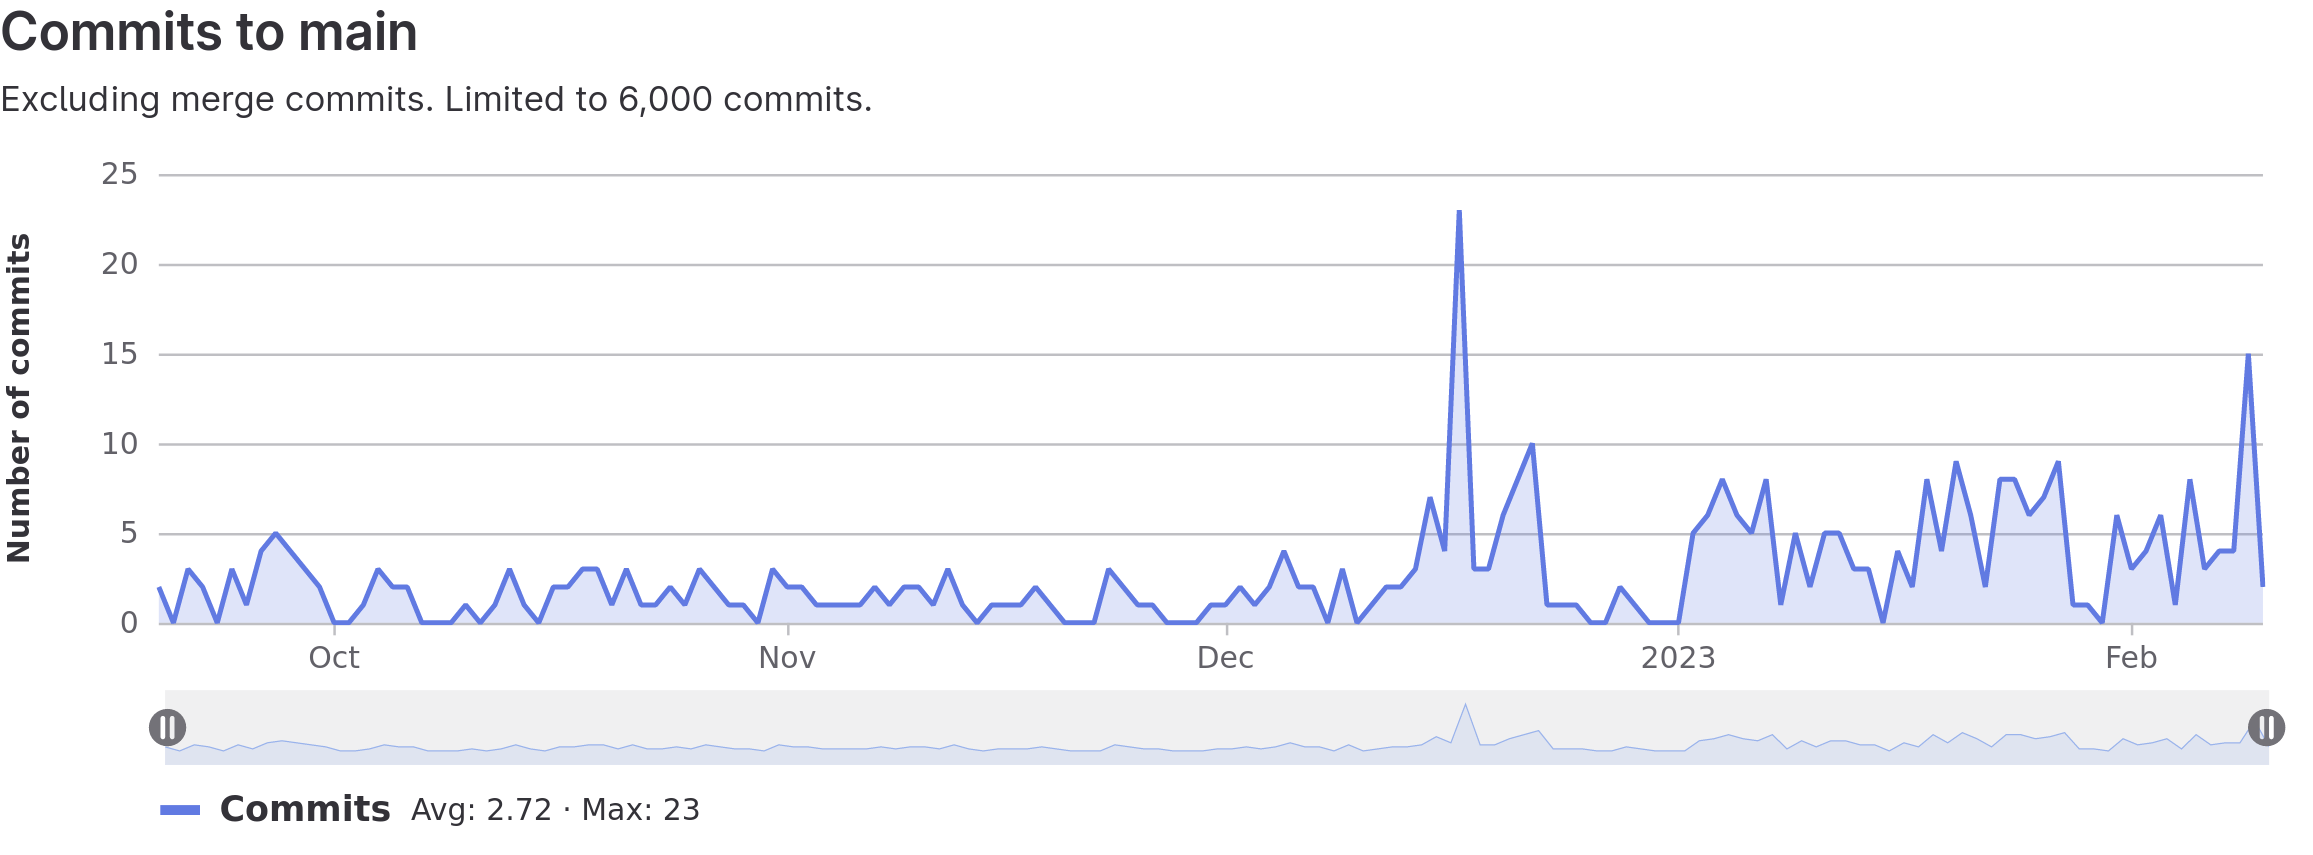
\includegraphics[width=1\textwidth]{03-tail/appendices/repository.png}

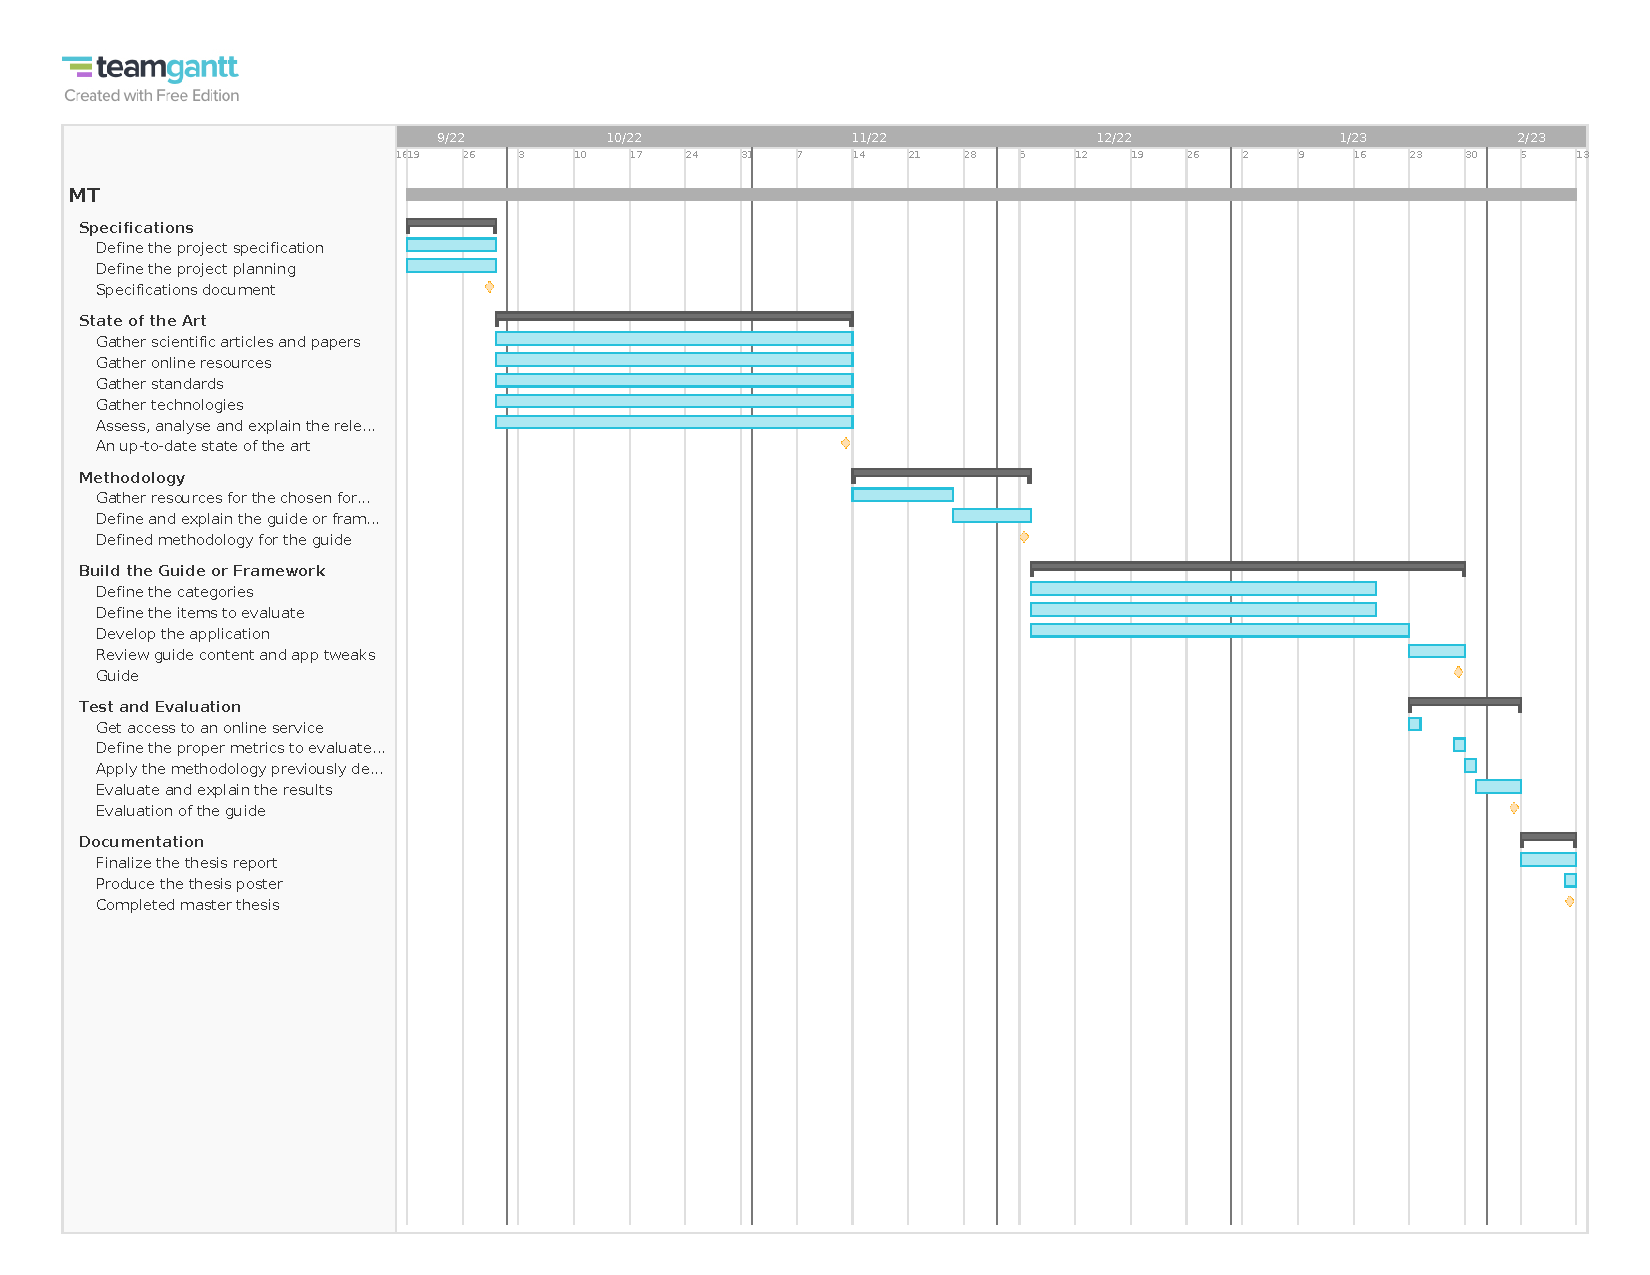
\includepdf[pages={-},angle=90]{03-tail/appendices/gantt_final.pdf}

% -----------------------------------------------------------------------------
\newappendix{Software and Tools}
\label{appendix:software}

This appendix does not list the software dependencies or tools if they have already been presented before in this report.

\subsection*{Office Tools}

All the software and tools used for the administrative or documentation tasks are listed here.

\citeproper{\LaTeX \ Suite - pdfTeX}, used to generate the documents for this project.

\begin{itemize}
	\item Version 3.141592653-2.6-1.40.22 (TeX Live 2021)
	\item Licence pdfTeX copyright, Lesser GNU General Public
\end{itemize}


\citeproper{Zotero}, used to manage the dissertation references.

\begin{itemize}
	\item Version 6.0.13
	\item Licence AGPL-3.0
\end{itemize}


\citeproper{Draw.io}, used to draw the different graphs.

\begin{itemize}
	\item Version 19.0.0
	\item Licence APACHE Licence, version 2.0
\end{itemize}


\citeproper{Microsoft Teams}, used to conduct organizational and follow-up sessions.

\begin{itemize}
	\item Version 1.5.00.10453 (64-bit) (64 bits)
	\item Licence Proprietary
\end{itemize}

\newpage

\subsection*{Development Tools}

All the software and tools used for the development tasks are listed here.

\citeproper{LibreWolf}, used for research, implementation and testing.

\begin{itemize}
	\item Version from 104.0.2-1
	\item Licence MPL-2.0 (d), GNU General Public Licence (GPL) et GNU Lesser General Public Licence (LGPL)
\end{itemize}


\citeproper{ungoogled-chromium}, used for research, implementation and testing.

\begin{itemize}
	\item Version 105.0.5195.125
	\item Licence BSD-3-Clause
\end{itemize}


\citeproper{GitLab}, used to manage the versioning of project resources.

\begin{itemize}
	\item Version GitLab Enterprise Edition 15.3.2-ee
	\item Licence MIT Licence
\end{itemize}


\citeproper{VSCodium}, used to implement \citeproper{JavaScript} software and to redact the \LaTeX documents.

\begin{itemize}
	\item Version 1.71.2
	\item Licence MIT Licence
\end{itemize}


\citeproper{PyCharm Professional}, used to implement the \citeproper{Python} script.

\begin{itemize}
	\item Version 2022.2.4
	\item Licence Copyright © 2010-2022 JetBrains s.r.o.
\end{itemize}


\citeproper{LibreOffice Calc}, used to create the spreadsheet file.

\begin{itemize}
	\item Version 7.4.3.2
	\item Licence MPL-2.0
\end{itemize}

% -----------------------------------------------------------------------------
% Back matter
% -----------------------------------------------------------------------------
\backmatter

% Bibliography
\cleardoublepage
\printbibliography[title={References}, heading=bibintoc]

% Glossary
\cleardoublepage
\phantomsection
%\addcontentsline{toc}{chapter}{Glossary}
\printglossaries

% TODO: Add index

% Add your CV here if you want

\end{document}

